\section{Mise en œuvre de la méthode de résolution par intervalles}



\subsection{Algorithmes}
L'algorithme de \emph{Branch and Prune} est au centre de la méthode de résolution par intervalles. Nous résumons ici ses deux étapes :  % met en oeuvre deux opérations détaillées dans \cite{Neumaier}: \\
%\begin{itemize}
%\item{Branch}
\paragraph{Branch :}
\begin{quote}\emph{Diviser pour mieux régner}\end{quote} Cette méthode consiste à diviser récursivement un problème en deux sous problèmes. Appliquée à la méthode de résolution par intervalles, on découpe en deux l'intervalle concerné (en son milieu ou non). On obtient alors deux problèmes plus \og petits \fg{} à étudier.%\clearpage
%\item{Prune}\\

\paragraph{Prune :}
La découpe d'un problème en sous problèmes peut amener à une situation ou un des sous problèmes créés ne contient aucune solution. On peut alors étudier et trier ces sous problèmes pour en supprimer les espaces de recherche superflus. Cette étape est appelée \emph{pruning}.

Au bout d'un certain nombre d'itération, l'algorithme de \emph{Branch and Prune} propose un ensemble de solutions sous la forme d'intervalles.% On visualise sur la figure \ref{fig:CercleDisque} un tel ensemble dans le cas d'une intersection entre un cercle et d'un disque.





\subsection{Données en sortie}
En sortie l'algorithme va nous retourner un ensemble de boîtes. Cet ensemble garantissant, à contrario des méthodes numériques classiques, que toutes les solutions y sont incluses. Dans la section \ref{par:out} un exemple d'illustration d'un tel ensemble est donné.

%~ \begin{figure}[h!] %on ouvre l'environnement figure
  %~ \center
%~ 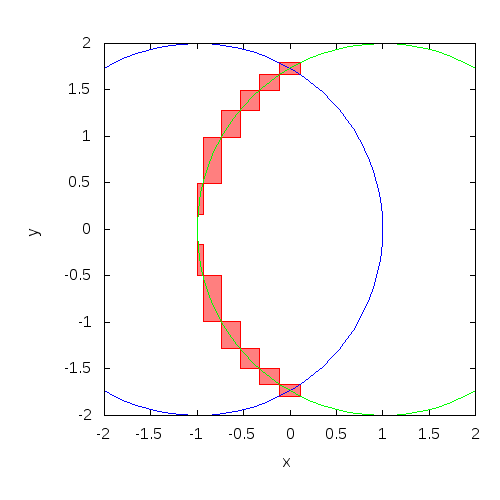
\includegraphics[scale=0.5]{img/circle-disk}
  %~ \caption{Intersection d'un cercle et d'un disque} %la légende
 %~ \label{fig:CercleDisque} %la légende
%~ \end{figure} %on ferme l'environnement figure

 Il est d'ailleurs possible de savoir si tout l'espace d'une boîte est solution du problème. En contrepartie on ne peut toujours garantir l'existence d'une solution dans une enveloppe, il peut donc exister une approximation autour des résultats de l'algorithme.

\clearpage
 
 \section{Applications par des outils}
\subsection{Realpaver}\label{realp}
Développé  au sein de l'équipe \textsc{OPTI}, cet outil reprend, entre autres, les méthodes de résolutions de contraintes géométriques par propagation d'intervalles. Il permet la résolution de systèmes d'équations à $n$ variables représentant des contraintes. Dans un soucis de précision ces solutions sont sous la forme d'intervalles \cite{realpaver}.% Les figures présentées dans ce chapitre (\ref{fig:Deuxcerlces}, \ref{fig:3Bconst} et \ref{fig:CercleDisque}), correspondent à des pavages calculés par cet outil. \cite{realpaver}.
\paragraph{Problème}
Soient deux disques, l'un de centre $(-1,0)$ et l'autre de centre $(1,0)$. Tous deux sont de rayon $2$. Donnez l'ensemble des solutions de l'intersection de ces deux disques.
\paragraph{Modèle}
L'outil \realpaver{}  modélise un tel problème de la sorte :
\label{realprob}
\begin{verbatim} 
Constants
  x0 = -1,
  y0 = 0,
  R0 = 2,
  x1 = 1,
  y1 = 0,
  R1 = 2
;
Variables
  x in ]-oo, +oo[,
  y in ]-oo, +oo[
;
Constraints
  (x-x0)^2 + (y-y0)^2 <= R0^2,
  (x-x1)^2 + (y-y1)^2 <= R1^2
;
\end{verbatim}
\paragraph{Données en sortie}\label{par:out}
L'ensemble de solutions suivant \realpaver{} propose l'ensemble de solutions suivant : 

\begin{verbatim}
RealPaver v. 0.4 (c) LINA 2004

INITIAL BOX
  x in ]-oo , +oo[
  y in ]-oo , +oo[

OUTER BOX 1
  x in [0.7924334198270921 , 0.795689483022687]
  y in [0.8806243697296342 , 0.8872330220900007]

...

OUTER BOX 3053
  x in [-0.7956894830226868 , -0.7924334198270919]
  y in [-0.8872330220900011 , -0.8806243697296345]

  precision: 0.00661, elapsed time: 150 ms

END OF SOLVING
  Property:     reliable process (no solution is lost)
  Elapsed time: 150 ms
\end{verbatim}
Ces 3053 solutions proposées par \realpaver{} sont illustrées sur la figure \ref{fig:DisqueDisque}.
\begin{figure}[ht!] %on ouvre l'environnement figure
  \center
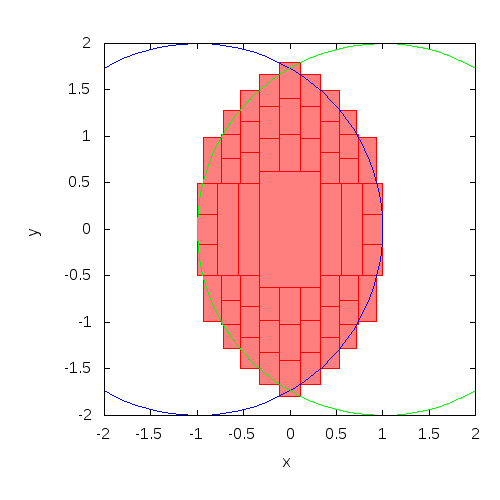
\includegraphics[scale=0.40]{img/disk-disk}
  \caption{Intersection de deux disques} %la légende
 \label{fig:DisqueDisque} %la légende
\end{figure} %on ferme l'environnement figure
\clearpage
\subsection{Autres outils existants}
\begin{description}
\item [CHOCO]  Projet commun  de l'École des Mines de Nantes, de \textsc{LIRMM} de Montpellier ansi que l'\textsc{INRA} de Toulouse. \textsc{CHOCO} est une librairie  \textsc{JAVA}  dédiée au résolution de \textsc{CSP} et à la programmation par contrainte. \cite{choco}
 \begin{figure}[h] %on ouvre l'environnement figure
  \center

\includegraphics[scale=0.50]{img/choco}
\end{figure} %on ferme l'environnement figure
\item [Google or-tools]
 Bibliothèque Python fournissant un solveur de contraintes générique et divers algorithmes, notamment sur les problèmes de graphes ou de sacs à dos : \cite{ortools}


\end{description}
